\chapter{Implementation Details}

% \begin{figure}{h}

% \end{figure}

After discussing requirements and simplified system models, this chapter discloses significant details of the implementation that powers FLOps.
We implemented FLOps mainly in Python.
Our goal is to use state-of-the-art tools for FLOps.
We analyzed and compared different open-source libraries and tools.

Table \ref{table:implementation_details_notion_subset} shows a heavily abbreviated subset of our internal comparison.
We refrain from exploring and discussing our findings to avoid bloating the thesis.
Especially because this landscape is constantly changing, and better options might exist since our analysis. 
We carefully considered every dependency that FLOps relies upon.
The dependency listings are available in the codebase \cite{flops_code}.

\begin{changemargin}{-1.5cm}{0cm}
    \centering
    \begin{tabular}{|M{3.0cm}||m{5.0cm}|c|c|c|m{4.0cm}|}
        \hline
            \textbf{Repository} & \textbf{Usage - Focus} & \textbf{Version} & \textbf{Issues} & \textbf{Stars} & Subjective Verdict \\
        \hline
        bprinty/ Flask-Authorize & Authorization \& Access & 0.2.7 & 9 & 64 & Too Small - “not mature” \\
        \hline
        python-restx/ flask-restx & API Development & 1.3.0 & 252 & 2k & Too many Open Issues \\
        \hline
        Flask-Middleware/ flask-security/ & Security for Flask Apps & 5.3.3 & 18 & 594 & SOTA for Security  \\
        \hline
        vimalloc/ flask-jwt-extended & JWT Support \& JSON Web Tokens & 4.6.0 & 9 & 1.5k & When JWT is required \\
        \hline
        flask-restful/ flask-restful & REST APIs & 0.2.12 & 98 & 6.7k & Outdated - Do not use \\
        \hline
        miguelgrinberg/ Flask-HTTPAuth &  Digest \& Token HTTP Authentication for Flask Routes & 4.8.0 & 9 & 1.2k & Seems good \\
        \hline
        dusktreader/ flask-praetorian & Security for Flask APIs (using JWT) & 1.5.0 & 4 & 339 & Small - Better Alternatives exist \\
        \hline
        lingthio/ Flask-User & Customizable User Authorization \& User Management & 1.0.2.2 & 99 & 1k & Outdated - No longer supported \\
        \hline
        pydantic/ pydantic &  Data Validation via Python Type Hints & 2.6.1 & 326 & 17.6k &  SOTA for Validation \& Serialization \\
        \hline
    \end{tabular}
    \captionof{table}{Subset of Internal Python Projects/Libraries Analysis (17.02.2024)} 
    \label{table:implementation_details_notion_subset}
\end{changemargin}


\section{User Interactions with the FLOps Manager}
This section details how users can interact with the FLOps manager.
It shows the currently available API endpoints and the SLA structure.

\subsection{API} \label{subsection:api}
We implemented the FLOps manager API via the Flask-OpenAPI3 framework \cite{framework:flask_openapi3}.
It is a relatively young and small framework that aligns Flask with OpenAPI3.
It uses Pydantic to verify data and automatically generate REST API and OpenAPI documentation that is compatible with popular frameworks such as Swagger.
We use Waitress \cite{waitress}, a production-quality WSGI server, to host the manager's API.

\subsubsection{Currently Available Endpoints}
\texttt{/api/flops/projects}\newline
This POST endpoint triggers a new FLOps project.
It expects users to provide a JSON SLA with the required project configurations and a bearer token authorizing the user on the orchestrator.
If no matching images exist, an image builder is created and deployed.
If an adequate image already exists, the request concludes straight away.
The user receives a confirmation that the new project has successfully started.
\vspace{5mm}
\newline
\texttt{/api/flops/tracking}\newline
The tracking endpoint allows users to spawn their personal tracking servers at will independently from an active project.
Usually, a tracking server is created during FL training.
This GET endpoint returns the tracking server / GUI URL.
\vspace{5mm}
\newline
\texttt{/api/flops/database}\newline
This DELETE endpoint only allows admins to reset the FLOps database.
Otherwise, the entire FLOps management suite needs a restart.
It returns a confirmation for the user.
\vspace{5mm}
\newline
\texttt{/api/flops/mocks}\newline
This POST endpoint creates mock data providers and deploys them on fitting learner machines.
We discuss these data providers later on in this thesis.
Similar to the project, this endpoint returns a confirmation to the user.
\vspace{5mm}
\newline

\pagebreak
\subsection{SLAs} \label{subsection:SLAs}
The FLOps manager can only instantiate a new project via an SLA.
This service layer agreement currently has the following structure.

% \begin{lstlisting}[language=json]
\begin{lstlisting}
    {
        % This key enables more verbose logging in the manager and project observer.
        "verbose": true, % default=false, optional
        % This ID should be the same as for the orchestrator.
        "customerID": "Admin", 
        % FLOps has only been tested for GitHub so far.
        "ml_repo_url": "https://github.com/Malyuk-A/flops_ml_repo_mnist_sklearn",
        % Supported flavors include: sklearn, pytorch, tensorflow, keras.
        "ml_model_flavor": "sklearn",
        % This key only works for special repositories intended for development.
        % It tells the builder to use prebuilt base images to significantly speed up image builds and development.
        "use_devel_base_images": false, % default=false, optional
        % This key expects a list of target platforms on which the built images should run.
        % It supports linux/amd64 and linux/arm64.
        "supported_platforms": ["linux/amd64"], % default=["linux/amd64"], optional
        "training_configuration": {
            % This key specifies the FL type.
            % FLOps supports classic and hierarchical modes.
            "mode": "classic", % default="classic", optional
            % Requested data tags should match available data on learner nodes.
            % Multiple different tags can be requested.
            % The ML data server will use local data fragments that match any of the provided tags.
            % If no data tags are provided the learner will notify watchers that it cannot find any data.
            "data_tags": ["mnist"],
            % Training cycles only apply to the hierarchical mode.
            "training_cycles: 1, % default=1, optional
            % This key tells learners the number of training and evaluation rounds to perform.
            "training_rounds": 3, % default=3, optional
            % Clients mean learners in this context.
            "min_available_clients": 2, % default=1, optional
            "min_fit_clients": 2, % default=1, optional
            "min_evaluate_clients": 2 % default=1, optional
        },
        % FLOps supports these two post-training steps.
        "post_training_steps": ["build_image_for_trained_model", "deploy_trained_model_image"], % default=[], optional
        % These are optional values that require fine-tuning.
        % Note that these values are not recommendations but placeholder values.
        "resource_constraints": {
            "memory": 250, % in MB
            "vcpus": 1,
            "storage": 25 % in MB
        }
    }
\end{lstlisting}

The following SLA shows a simple classic FL project configuration with both post-training steps enabled.
It requires two learners for training.

\begin{lstlisting}[language=json]
    {
        "verbose": true,
        "customerID": "Admin",
        "ml_repo_url": "https://github.com/Malyuk-A/flops_ml_repo_mnist_sklearn",
        "ml_model_flavor": "sklearn",
        "training_configuration": {
            "data_tags": ["mnist"],
            "min_available_clients": 2,
            "min_fit_clients": 2,
            "min_evaluate_clients": 2
        },
        "post_training_steps": ["build_image_for_trained_model", "deploy_trained_model_image"],
    }
\end{lstlisting}

The next SLA displays a more advanced configuration with HFL, multi-platform support, and more FL actors.

\begin{lstlisting}[language=json]
    {
        "customerID": "Admin",
        "ml_repo_url": "https://github.com/Malyuk-A/flops_ml_repo_cifar10_pytorch",
        "ml_model_flavor": "pytorch",
        "supported_platforms": ["linux/amd64", "linux/arm64"],
        "training_configuration": {
            "mode": "hierarchical",
            "data_tags": ["cifar10"],
            "training_cycles": 10,
            "training_rounds": 5,
            "min_available_clients":3,
            "min_fit_clients": 3,
            "min_evaluate_clients": 3
        },
        "post_training_steps": ["build_image_for_trained_model", "deploy_trained_model_image"],
    }
\end{lstlisting}

\section{Image Building}

From our understanding the automatic image build process that turns user ML code into FL-capable containerized multi-platform images is one of the major novel contributions of this work.
This process is a non-trivial endeavor requiring advanced understanding and application of various domains.
This chapter is dedicated to analyzing these required synergies.
Firstly, it elaborates on the need to build these images and explains related challenges.
Secondly, it discusses different approaches and their limitations in building images in the given environment.
Thirdly, this chapter showcases details about internal FLOps image builder processes.
The last subsection explains how FLOps handles multi-platform image builds.

\subsection{Dependency Management}

The goal of using containerized images is to avoid the need and struggle to set up and configure machines individually.
This setup and configuration part is especially crucial for ML workloads.
Many different ML frameworks and libraries exist and need to cooperate with other software tools.
These tools cover various aspects of ML, ranging from unsupervised to supervised learning.
Subfields include clustering, reducing feature spaces, classification, regression, and neural networks.
Just neural networks as a field represent a multifaceted domain that requires different tools.
Neural networks span from simple nets with a single hidden layer to deep neural networks, convolutional networks, transformers, and many more.
Besides targeting different ML disciplines, they can be fine-tuned for specific environments, such as massive supercomputers, end-user work machines, or IoT and edge devices.
Popular tools include TensorFlow, Keras, PyTorch, and Scikit-learn, which all have different extensions and forked projects.
Even small basic ML projects can already contain several hundred dependencies.
All of these tools have different versions and require careful consideration and version management to avoid unexpected side effects and errors.

We elaborated in section \ref{subsection:fl_research} that the relevant literature rarely touches upon the initial device configuration and setup.
Most authors assume that these dependencies are already properly installed and configured on the devices.
Many works in FL discuss and propose better ways of selecting and distributing training loads and model parameters (\ref{subsection:fl_research}).
They also omit the aspects of dependencies.
Before it is possible to train a model via FL or ML, the device needs to have all the necessary capabilities correctly configured.
Containers resolve most of these issues, especially for heterogeneous devices and environments.
These reasons motivated us to develop and include automatic image-build processes.

Conventionally, ML workflows are implemented in Python.
Therefore, the mentioned dependencies are handled via Python's own package repository, PyPI (Python Package Index).
These packages are usually installed and managed via Python's package installer pip.
These standard tools display weaknesses when resolving dependencies in extensive projects.
It can happen that pip fails to resolve and properly install the dependencies in a compatible way.
Additionally, because pip is implemented in Python, which is not the fastest programming language, this dependency resolution can take a long time.
Other tools try to resolve these weak points.

A popular alternative to pip is the Conda suite.
Conda \cite{docs:conda} is an open-source package and environment manager that is popular with ML and Data engineers.
It focuses on Python but supports other languages as well.
Conda provides and enables convenient virtual Python environments and resolves dependencies more successfully and quickly than pip.
Anaconda \cite{docs:anaconda} is Conda's Python distribution that includes Conda and comes with more than 100 commonly used packages.
This distribution is heavy-weight and unfit for lightweight, containerized, or CI workflows.
Miniconda \cite{docs:miniconda} is a minimal Anaconda version that only includes Conda and a small mandatory set of dependencies.
It is ideal for lightweight environments that should only include necessary (custom) dependencies.
Conda is also implemented in Python.
Thus, the dependency resolution process speed remains a bottleneck.
Mamba \cite{docs:mamba} is a reimplementation of Conda in C++.
This allows Mamba to resolve dependencies a significantly faster than Conda.
Similarly to Miniconda, Micromamba \cite{docs:micromamba} is a minimal distribution of Mamba.

Additionally, there is no single unified source for packages or standard for building such packages.
Various package servers, mirrors, channels, and package builders exist.
One example is Conda-Forge.
Furthermore, the structure, build, and publish processes for Python packages have changed vastly over the years.
Native Python only recently switched to a more homogeneous approach via pyproject.toml files \cite{setuptools_userguide}.
Previously setup.py and setup.cfg files were used for these purposes.
In addition, there are other tools like Poetry \cite{docs:poetry} or the very new and lightning-fast uv \cite{uv} manager that is implemented in Rust.
In conclusion, Python's dependency management ecosystem is vast and complex.
The newer a tool, the quicker it tends to be, but it also lacks sophisticated maintenance and might not support all necessary packages or versions.

FLOps should support as many projects and dependencies as possible.
For this reason, FLOps uses miniconda.
It supports different Python versions, easily resolves and handles dependencies, and is a lightweight solution.
Conda now also supports multiple different dependency resolvers.
Since the end of 2023, Conda has been using the libmamba resolver by default, which uses Mamba \cite{docs:conda_libmamba}.
Therefore, FLOps uses a fast and reliable dependency resolver.

Besides the complexity of Python's dependency landscape, ML dependencies can be huge.
\begin{figure}[t]
    \begin{changemargin}{0cm}{0cm}
        \centering
        \begin{tabular}{|c||c|c|c|c|}
            \hline
                \textbf{Image} & python:3.12.4 & python:3.12.4-slim & anaconda3:latest & miniconda3:latest \\
            \hline
                \textbf{Size} & 1.02 GB & 133 MB & 4.5 GB & 611 MB
            \\
            \hline
        \end{tabular}
        \captionof{table}{Conda Python Image Size Comparison (29.08.2024)} 
        \label{table:conda_python_comparison}
    \end{changemargin}
\end{figure}
Table \ref{table:conda_python_comparison} shows four pulled images and their sizes.
All images use Python version 3.12.4.
The default Python image is one GB in size.
Its official slim alternative is almost ten times smaller.
The full anaconda image has 4.5 GB.
The miniconda image is more than seven times smaller than the full anaconda version but more than five times larger than the slim Python image.
Note that these are the pulled docker image sizes, not the compressed registry ones.
(The Conda images are from the official continuumio project.)

Table \ref{table:ml_libs_images_compared} shows a selection of pulled images of popular ML tools.
All images are the latest official images by the ML tool providers, except scikit-learn.
These images can vary enormously in size.
Some of them require several GBs of disk space and bandwidth to pull.
Any FLOps image built on top of these dependencies will be even larger due to the additional FL and MLOps dependencies.

\begin{figure}[t]
    \begin{changemargin}{0cm}{0cm}
        \centering
        \begin{tabular}{|c||c|c|c|}
            \hline
                \textbf{Image} & smizy/scikit-learn-docker & tensorflow/tensorflow & pytorch/pytorch \\
            \hline
                \textbf{Size} & 515 MB & 1.86 GB & 7.6 GB
            \\
            \hline
        \end{tabular}
        \captionof{table}{A selection of popular ML library images and their sizes (29.08.2024)} 
        \label{table:ml_libs_images_compared}
    \end{changemargin}
    \end{figure}

\subsection{Image Builders} \label{subsection:image_builders}

The most popular and widespread containerization tool is Docker.
It is also preferred when building images.
Usually, building images via Docker is straightforward.
One creates a Dockerfile and runs Docker commands to build a new image on a host machine based on this file.

FLOps requires a more complex approach to build images.
Its image builder is a service running on a worker node that Oakestra orchestrates.
This service is a containerd container.
It is not possible to simply run docker in such an environment to build images.
The critical issue here is that docker cannot be run trivially in another container due to restricted privileges and access to host system capabilities \cite{paper:dind}.
A popular workaround, especially for CI/CD workloads, is called Docker in Docker (DinD) \cite{paper:dind}.
Many CI/CD tools support DinD natively.
One example includes GitLab's CI/CD.
Setting up and using DinD manually on a host machine is non-trivial and error-prone.
Getting docker to work inside managed Oakestra containers is even more challenging.
One significant reason for these issues is that docker requires its daemon to run for building images.
Nested Docker daemons are a complicated matter \cite{paper:dind} that can require significant adjustments to how the orchestrator coordinates containerization on worker nodes.
For example, the orchestrator could require worker nodes to mount their docker sockets to the container, which would lead to further security risks.

The only functionality that FLOps requires here is building images inside containers, not executing them from within.
There exist various alternatives to Docker that specialize in building containerized images.
Thanks to the coordinated efforts of the OCI \cite{open_container_initiative} and others, these tools all build compatible images.
Alternative tools include kaniko, Podman \cite{docs:podman}, and Buildah \cite{buildah_homepage}.
FLOps uses Buildah.

Buildah is an open-source daemon-free tool that specializes in building OCI-compliant images.
It can run on host machines or inside containers.
It features many equivalent Docker commands and supports building images step-wise, programmatically, or via Dockerfiles.
Red Hat released Buildah initially in 2017, and its first major version was released in 2018.
Podman and Buildah are complementary tools that have some shared documentation and aspects.
Great resources to find out more about Podman, Buildah, and their relationship are available here \cite{redhat_docs:podman,redhat_docs:buildah,buildah_vs_podman}.

It was challenging to make container-internal image-building work for FLOps via Oakestra.
This image build process is especially complicated because it performs heavy dependency resolutions and installations.
We needed to add a new optional flag to Oakestra deployments that enabled to mount /dev/fuse.
The FUSE userspace filesystem framework enables non-privileged and secure mounts \cite{docs:fuse_linux_kernel}.
In addition, Buildah has to build its images with the chroot isolation flag enabled.
As a result, FLOps uses a highly fine-tuned and optimized builder environment that enables it to build images inside containers of orchestrated worker nodes.

Furthermore, we put a lot of thought and time into refining and polishing FLOps' docker files.
They build the foundation for all FLOps components, from project services and management components to auxiliary containers.

\subsection{FLOps Image Builder Details}

This subsection showcases how the FLOps image builder service concretely builds its different images.
The following expands upon Figure \ref{fig:flops_simple_image_builder} from \ref{subsection:flops_overview}.

\begin{figure}[p]
    \begin{adjustwidth}{-0.1\paperwidth}{-0.1\paperwidth}
        \centering
        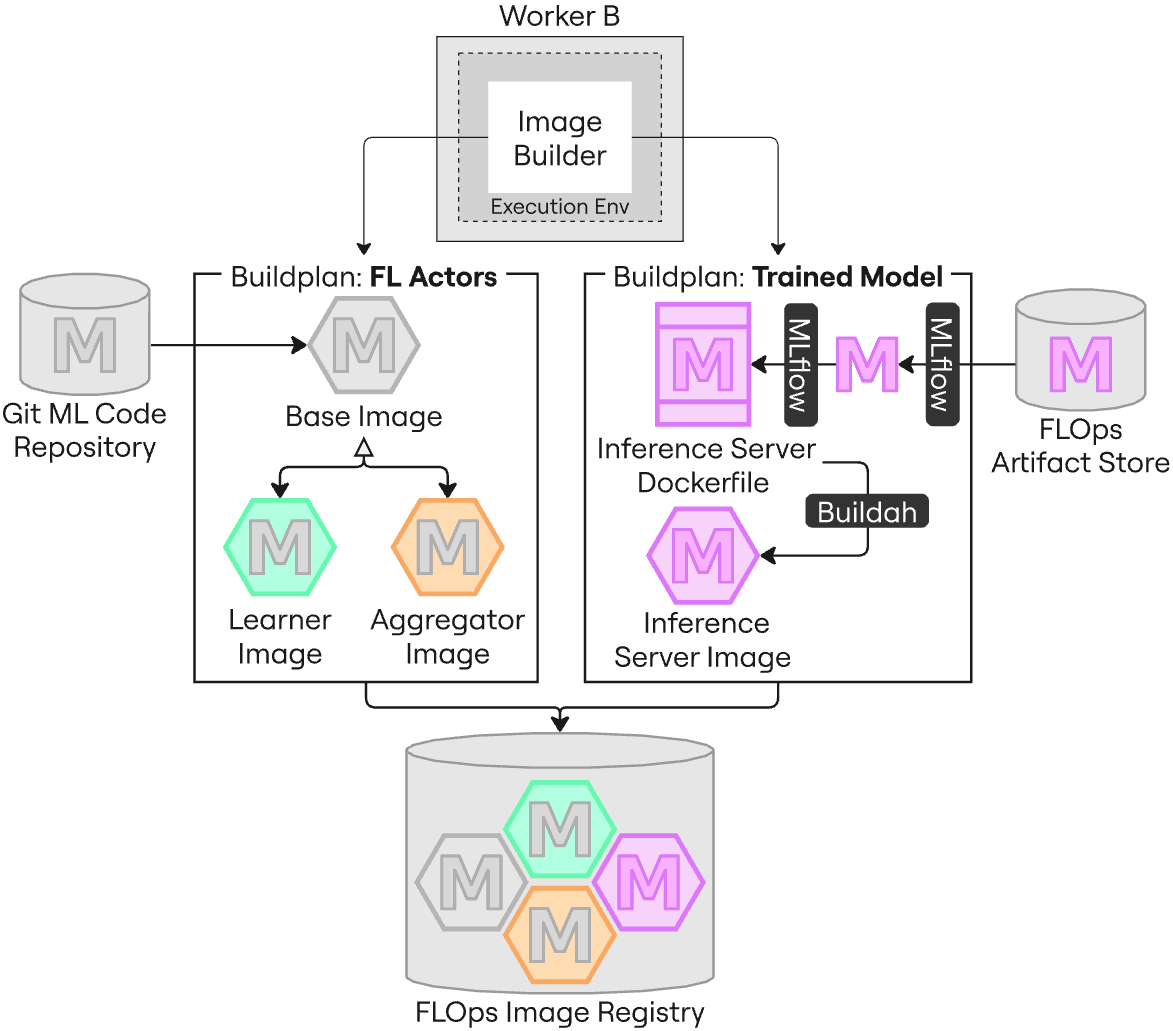
\includegraphics[width=0.80\paperwidth]{detailed_builder.png}
        \caption{Detailed FLOps Image Builder Processes}
        \label{fig:detailed_builder}
    \end{adjustwidth}
\end{figure}

Figure \ref{fig:detailed_builder} depicts the details how FLOps Image Builder works.
The grey Ms represent the untrained model (structure).
Purple Ms stand for the trained model.
Hexagons symbolize container images.
The service tracks the time different steps take and returns to the FLOps manager a summary of its total runtime and the runtime of individual steps.
The image builder supports two different build plans.

The first step in the FL Actors build plan is to fetch the user's ML code from his specified repository.
Secondly, the service builds a base image that contains all dependencies common to the learner and aggregator.
Due to the current multi-platform solution, the service pushes the base image to the image registry hosted in FLOps management.
Building and pushing the base image take up most of the service's total runtime.
The service continues to build the FL actor images one after another, pushing them in the end.
Thanks to the base image, these steps are relatively quick.
Pushing the base image does not generate meaningful overhead because of image layer caching.
The FL actor images reuse all the base image layers.
Thus, pushing them is accelerated, and the image registry recognizes and reuses its base image copy's layers.

Flower's design does not require the aggregator to possess any information about the model, including its structure or dependencies.
The aggregator's job is to average the received model parameters.
This process is based on simple mathematics and requires no other model-specific information or dependencies.
Therefore, the aggregator image and node can be relatively lightweight compared to the learners.
However, logging the trained model via MLflow requires access to the complete trained model, especially its structure.
The corresponding dependencies are necessary because a model structure is defined in a concrete ML framework.
Therefore, FLOps explicitly also includes these dependencies and the model structure in the aggregator.
During FL training only the model parameters are transmitted.
The aggregator's model copy is only needed at the very end of training.
The aggregator populates its untrained model copy via its final global model parameters.
This populated model gets logged.
Note that the model structure is initially defined in the user's ML repository and can be easily cloned and injected into images via the builder service.

The trained model build plan can only be run after the FL training is completed and the trained model is saved in the artifact store, which is hosted in the FLOps management.
MLflow provides commands to turn stored models into containers \cite{docs:mlfow_docker_cmds}.
The issue with this approach is that MLflow only provides this capability via Docker for all these commands, including building.
This approach works well directly on host machines but not inside containers (\ref{subsection:image_builders}).
As a workaround, FLOps uses MLflow to pull the stored trained model into the builder container.
Then, the service uses MLflow again to create a dockerfile based on this model.
FLOps' builder service augments this dockerfile to support multiple platforms and builds the trained model image via Buildah.
This built image wraps the trained model via an inference server.
One optional FLOps post-training step deploys this inference server directly after the builder service terminates.

\begin{figure}[b]
    \begin{changemargin}{0cm}{0cm}
        \centering
        \begin{tabular}{|c||c|c|c|c|c|c|}
            \hline
                \textbf{Image} & Image Builder & MLflow & Client & Server & SuperNode & SuperLink \\
            \hline
                \textbf{Size} & 3.0 GB & 819 MB & 1.16 GB & 1.13 GB & 232 MB & 232 MB
            \\
            \hline
        \end{tabular}
        \captionof{table}{Important FLOps Image Sizes (30.08.2024)} 
        \label{table:relevant_image_sizes_for_building}
    \end{changemargin}
\end{figure}

Table \ref{table:relevant_image_sizes_for_building} shows the sizes of different relevant images to provide more context for the final results and build processes.
The Image Builder image is the FLOps builder service.
It is noteworthy that FLOps' builder service without the MLflow (2.12.1) dependency is 900 MB and the official MLflow image is 819 MB.
The increase of more than 2.4 GB only due to this dependency is worth investigating.
The remaining images from the table are all from Flower \cite{flower_images}.
Flower recently introduced a significant change (Flower Next API \cite{docs:flower_next}) in how they use FL clients and servers.
They plan to deprecate the old approach that FLOps is using.
We tried migrating to the new Flower paradigm but encountered several issues with our current implementation.
Explaining Flower Next and FLOps' challenges with it would bloat this thesis.
This aspect is a great topic for future FLOps improvements.
The client and server images from the table are deprecated.
Their new replacements are the SuperNode and SuperLink, which are significantly smaller.
We mention these images to compare them with FLOps' FL actor images.

\begin{figure}[t]
    \begin{changemargin}{0cm}{0cm}
        \centering
        \begin{tabular}{|c|c|c|c|c|c|}
            \hline
                \textbf{Standalone} & \textbf{Base} & \textbf{Learner} & \textbf{Aggregator} & \textbf{Total Process} & \textbf{Base Image Build} \\
            \hline
                515 MB & 2.79 GB & 2.79 GB & 3.55 GB & 6min 20s & 3min 53s
            \\
            \hline
        \end{tabular}
        \captionof{table}{Simple Scikit-learn MNIST Build Example} 
        \label{table:sklearn_mnist_build_example}
    \end{changemargin}
\end{figure}
Table \ref{table:sklearn_mnist_build_example} shows a singular example of running a FLOps project using Scikit-learn and the MNIST dataset.
The Standalone refers to the standalone Scikit-learn image from Table \ref{table:ml_libs_images_compared}.
The base and learner images are equally large because the learner image only changes the files it works with but reuses all dependencies from the base image.
Therefore, the aggregator has a superset of the learner dependencies.
The total execution time for the builder service took 6 minutes and 20 seconds.
The base image build alone took almost four minutes.

FLOps Management uses and hosts an instance of the open-source CNCF (Cloud Native Computing Foundation) Distribution Registry \cite{docs:cncf_distribution_registry}.
This registry allows FLOps to be independent of any other registry provider.
FLOps has complete control and immediate access to this registry.


\subsection{Multi-Platform}

This subsection explains how FLOps builds multi-platform images.
Usually, end users build images only for a single platform.
Their builder knows their host's architecture and uses it as a target platform.
When inspecting popular public images, they support multiple target platforms.
Each image tag can have multiple digests, each representing a different platform.
For example, the latest Alpine image \cite{alpine_multiplatform_image} supports at least linux/amd64 and linux/arm/v6.
By default, it is impossible to run images that are intended for different architectures on machines with incompatible host architectures.
Specific workarounds via emulation exist.

The key of building and referencing images that support multiple platforms are manifests.
A plain manifest file contains information about a unique image digest.
This information includes its media type, size, layers, and architecture.
When an image supports multiple platforms, it has multiple digests, thus one manifest per digest.
Image indexes were invented to group these different manifests.
Note that image indexes refer to the OCI standard term \cite{oci_image_index}.
In Docker, they are called fat manifests or manifest lists \cite{docs:docker_manifest}.
As a result, different host architectures can use the same image tag and pull their matching digest image.
This happens because the local builder reads the image index and picks a suitable manifest.
Examples for manifests are available here \cite{docs:docker_manifest}.

Multi-platform images are a deep topic.
Because of its rapid development, many different media types, versions, and schemas for manifests exist.
Build machines need to use the same conventions as their image registries.
Discussing these details here would lead to bloat.
Excellent information about this topic is available here \cite{docs:image_manifest_versions_schemas}.

Previously, one had to manually build one image per target architecture on a machine of that architecture, provide the image tag with an architecture suffix, and push it.
Once all these different images were pushed, an image index had to be created and pushed.
Nowadays, a convenient solution for building multi-platform images is using docker's buildx builder \cite{docs:docker_buildx}.
It can build and push multi-platform images concurrently with a single command.

The FLOps image builder does not use docker to build its images (\ref{subsection:image_builders}).
Buildah also supports building multi-platform images but lacks the convenient new features of docker's buildx.
From our experience, Buildah lacks sufficient documentation regarding building and pushing multi-platform images.
We needed to look into its source code, read other sources, and experiment extensively until we made this work.

Another significant requirement for building multi-platform images on a single machine is emulating other architectures.
Otherwise, only images for the host's architecture can be built.
It is also possible to cross-compile or use multiple dedicated builder nodes with proper architectures \cite{docs:docker_multiplatform_image_builds}.
Conventionally, QEMU \cite{docs:quemu} is used to emulate such tasks.
Docker Desktop includes QEMU for Mac and Windows by default \cite{docs:docker_multiplatform_image_builds}.
QEMU translates the requested target architecture instructions into ones the host machine can understand.
Due to FLOps' special circumstances, which involve building complex images in orchestrated, containerd containers on heterogeneous devices, various approaches seem to be available to realize emulation.
Ideally, the emulator would be part of the builder image, thus avoiding the need to modify or require anything from the worker nodes.
After many unsuccessful attempts, we decided to require worker nodes that should build multi-platform images to pre-install QEMU.
For Linux machines, this can be done by installing an open-source package called qemu-user-static.

In conclusion, using this approach, the FLOps builder service can build multi-platform images.
All other FLOps (static) images, including the builder service or project observer, are also available for linux/amd64 and linux/arm64.
For example, all these images can be started on a Raspberry Pi 4, but these devices seem to lack sufficient resources to handle the FL training.
An additional downside of multi-platform image builds comes with the slowness of emulation.

Table \ref{table:sklearn_mnist_multi_platform_build_example} shows a simple example of FLOps' builder service's build times for different platforms.
The build machine natively supports linux/amd64.
Therefore, this build is much faster than the emulated arm one.
Both rows show the build times when only a single platform is requested.
The build times would be combined to support both platforms simultaneously.

\begin{figure}[t]
    \begin{changemargin}{0cm}{0cm}
        \centering
        \begin{tabular}{|c|c|c|c|c|c|c|}
            \hline
            \textbf{Builder Architecture} & \textbf{Target Platform} & \textbf{Full Build} & \textbf{Base Image} & \textbf{Actor Images} \\
            \hline
            linux/amd64 & linux/amd64 & 4min & 2min 30s & 1min 30s \\
            \hline
            linux/amd64 & linux/arm64 & 18min & 12min & 6min \\
            \hline
        \end{tabular}
        \captionof{table}{Simple Scikit-learn Multi-Platform Build Times Example} 
        \label{table:sklearn_mnist_multi_platform_build_example}
    \end{changemargin}
\end{figure}




\section{Local Data Management}

This section explains how FLOps handles local data on learner nodes.
Firstly, it covers what kind of data and datasets suit FL and why.
Secondly, it discusses how state-of-the-art projects in the industry handle enormous amounts of data for ML and Big Data applications.
Thirdly, it explores how exactly FLOps manages the local data and what architecture it uses for this task.
The last subsection showcases FLOps' mock data provider service, which makes development and testing more convenient.

\subsection{Appropriate Data for FL}

FL, especially cross-device FL, specializes in massive numbers of heterogeneous devices with diverse non-IID data.
For FL, one can use conventional datasets, such as MNIST or CIFAR10.
However, such homogeneous and IID data is not representative of data found on real devices.
Many works in the field of FL specialize and compare how well they perform on non-IID data (\ref{subsection:fl_research}).
For this reason, various datasets and benchmarks have been created explicitly for FL.
One recurring prominent FL benchmarking tool is LEAF \cite{paper:leaf_fl_benchmark}.
It does not solely specialize in FL but in more general federated settings.
It includes several implementations and datasets.
As mentioned in Table \ref{table:fl_research_table_2}, we had little success working with this benchmark.
This finding is noteworthy because LEAF seems to be the primary and sole source for the FEMNIST dataset, which many FL papers mention and use for evaluation.

FEMNIST seems to be one of the most popular dedicated FL benchmarking datasets.
It is a federated version of the Extended MNIST (EMNIST \cite{emnist_dataset}) dataset.
FEMNIST splits the EMNIST dataset into multiple classes or data partitions based on individual (digit/symbol) writers.
Extended projects exist that wrap the access to FEMNIST via the high-speed HDF5 binary data format \cite{hdf5_femnist}.
The FEMNIST dataset is a prominent example of many dedicated FL datasets and benchmarks.
A detailed listing and comparison of other similar resources is available in \cite{thesis:tum_fl_framework_comparison}.

FLOps requires a convenient way of accessing suitable data for development and testing purposes.
Our experience trying out LEAF taught us that using these dedicated datasets can be challenging and error-prone.
Instead of figuring out how to unify these different dedicated FL datasets and benchmarks, we use Flower Datasets \cite{flower:datasets}.
We already discussed Flower Datasets briefly in \ref{subsection:flower}.
The vital thing to know about this young project is that it uses and splits up Hugging Face datasets into non-IID data fragments.
It enables users to turn conventional ML datasets into FL-optimized ones.
Users can configure this approach freely.

\subsection{ML \& Big Data Formats}

The field of Big Data and ML formats is vast and complex.
It provides many insights into different optimization approaches.
Great resources to find out more are available here \cite{influxdb_apache_stack,apache_arrow_flight_sql_2022,columnar_roadmap_parquet_and_arrow,apache_arrow_flight_intro}.
The following are significant takeaways after investigating this domain.
\vspace{5mm}
\newline
\textbf{Managing Big Data is a booming Field}\newline
Storing and handling Big Data is a massively popular, expensive, and profitable business that regularly attracts hundred-million-dollar investments.
This environment leads to healthy competition, solid standards, and bold advancements in the field.
\vspace{5mm}
\newline
\textbf{Reuse}\newline
Data management and optimizations are universally needed.
These areas have several decades of solid research to back up best practices and avoid known pitfalls.
Similarly to security, one should avoid reinventing and reimplementing foundational features from the ground up.
Instead, it is recommended that existing open-source industry-favored solutions be reused.
\vspace{5mm}
\newline
\textbf{(De)Serialization is a critical Bottleneck}\newline
When each subsystem has its own internal memory format, significant amounts of CPU work get wasted on (de)serialization.
The recommended way to avoid this is to stick to a uniform format.
The more tools support such a uniform format, the easier and faster cooperation, communication, and transmission can be.
\vspace{5mm}
\newline
\textbf{Big Data and ML Data should use Columnar Formats}\newline
Usually, dataset features are split up into different columns.
These features can be diverse and require different data types for storage.
When storing and handling conventionally stored row-wise data, all these different data types and features complicate and slow down processing.
Instead, if the data is stored and handled column-wise, advanced optimizations, and compressions can handle homogeneous features and their data type.
As a result, the same data can be processed more compactly and faster.
\vspace{5mm}
\newline
The sources above recommend the following open source state-of-the-art formats and technologies.
All of them are from Apache.
\vspace{5mm}
\newline
\textbf{Arrow}\newline
Arrow is a language-agnostic columnar memory format.
It is optimized for modern CPUs and GPUs.
It supports zero-copy reads, which avoid serialization and accelerate data access.
Arrow is especially popular for interoperability.
This format should be used for data in memory. \cite{arrow_repo} 
\vspace{5mm}
\newline
\textbf{Parquet}\newline
Parquet is also a columnar file format.
Its focus is on efficient data storage and retrieval.
Its benefit over Arrow is that it needs less space due to its special compression and encoding.
This format should be used to store data on disks. \cite{docs:parquet}
\vspace{5mm}
\newline
\textbf{Arrow Flight}\newline
Arrow Flight is a gRPC-based framework.
It supports parallel data streams.
When used with compatible data, it overcomes (de)serialization overheads and speeds up data transfer.
Flight should be used to transport Apache formatted data over the network. \cite{docs:arrow_flight}
\vspace{5mm}
\newline
The last subsection mentioned that FLOps uses Flower Datasets, which uses Hugging Face Datasets underneath.
Hugging Face Datasets use Arrow \cite{docs:hugging_face_arrow}.
Therefore, the findings in this subsection are directly applicable and relevant to FLOps.

\subsection{FLOps' Local Data Management Architecture}
\begin{figure}[h]
    \begin{adjustwidth}{-0.1\paperwidth}{-0.1\paperwidth}
        \centering
        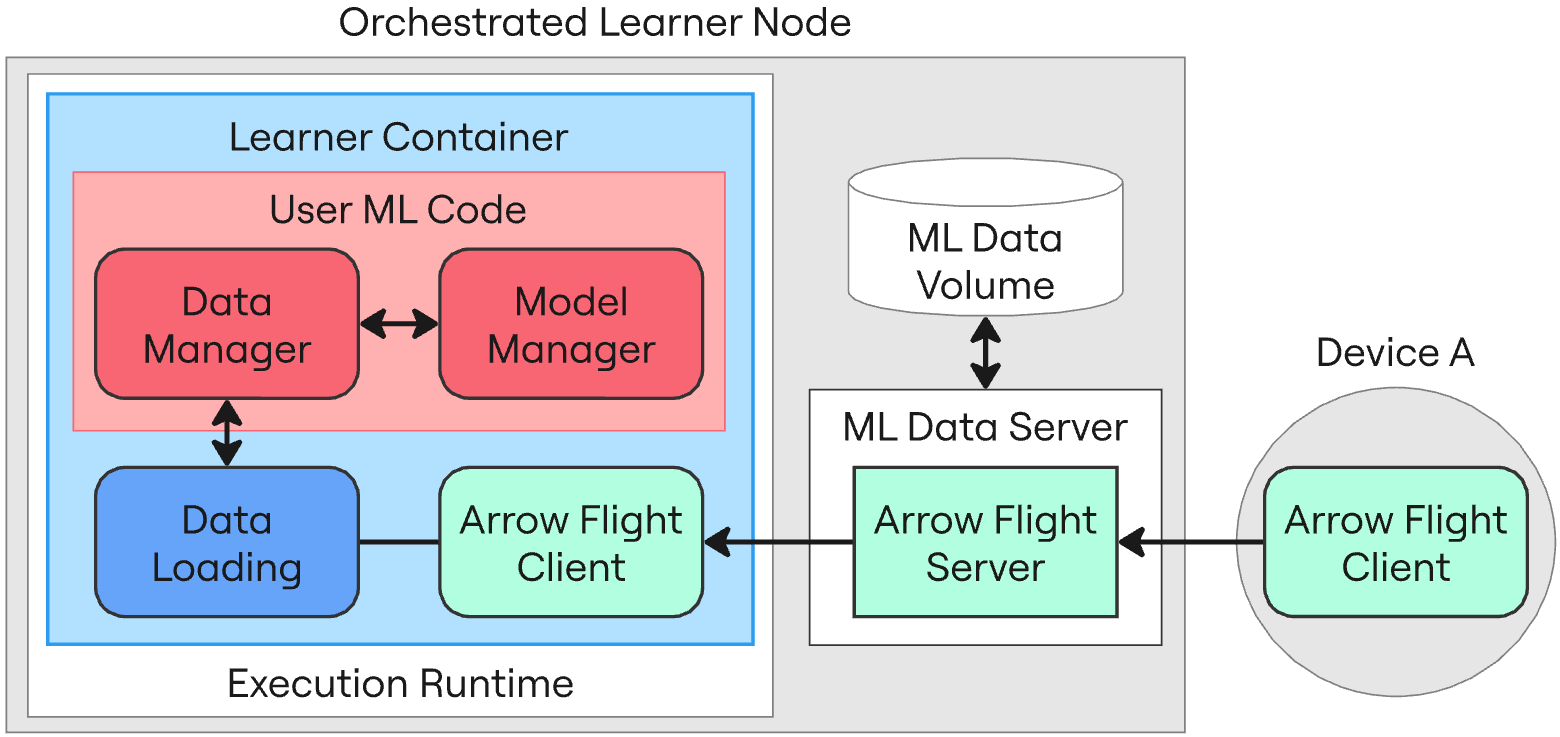
\includegraphics[width=0.80\paperwidth]{local_data_loading_medium.png}
        \caption{FLOps Local Data Management Structure}
        \label{fig:medium_local_data_management}
    \end{adjustwidth}
\end{figure}
Figure \ref{fig:medium_local_data_management} depicts the architecture of FLOps' local data management.
The important concretions compared to the simplified version in Figure \ref{fig:flops_simple_data_management} from \ref{subsection:flops_overview} are as follows:
The learner container and the data-providing device must have an Arrow Flight client installed and connected to the Arrow Flight server in the ML data server.
The data loading component in the learner uses the Flight client to retrieve the matching data.
It gets added by the builder service and is not part of the user's ML code.
The data and model manager utilize this loaded data.
Note that the figures in this subsection depict a single data source device for optimizing page space.
Arbitrary many devices are supported by this setup.

\begin{figure}[p]
    \begin{adjustwidth}{-0.1\paperwidth}{-0.1\paperwidth}
        \centering
        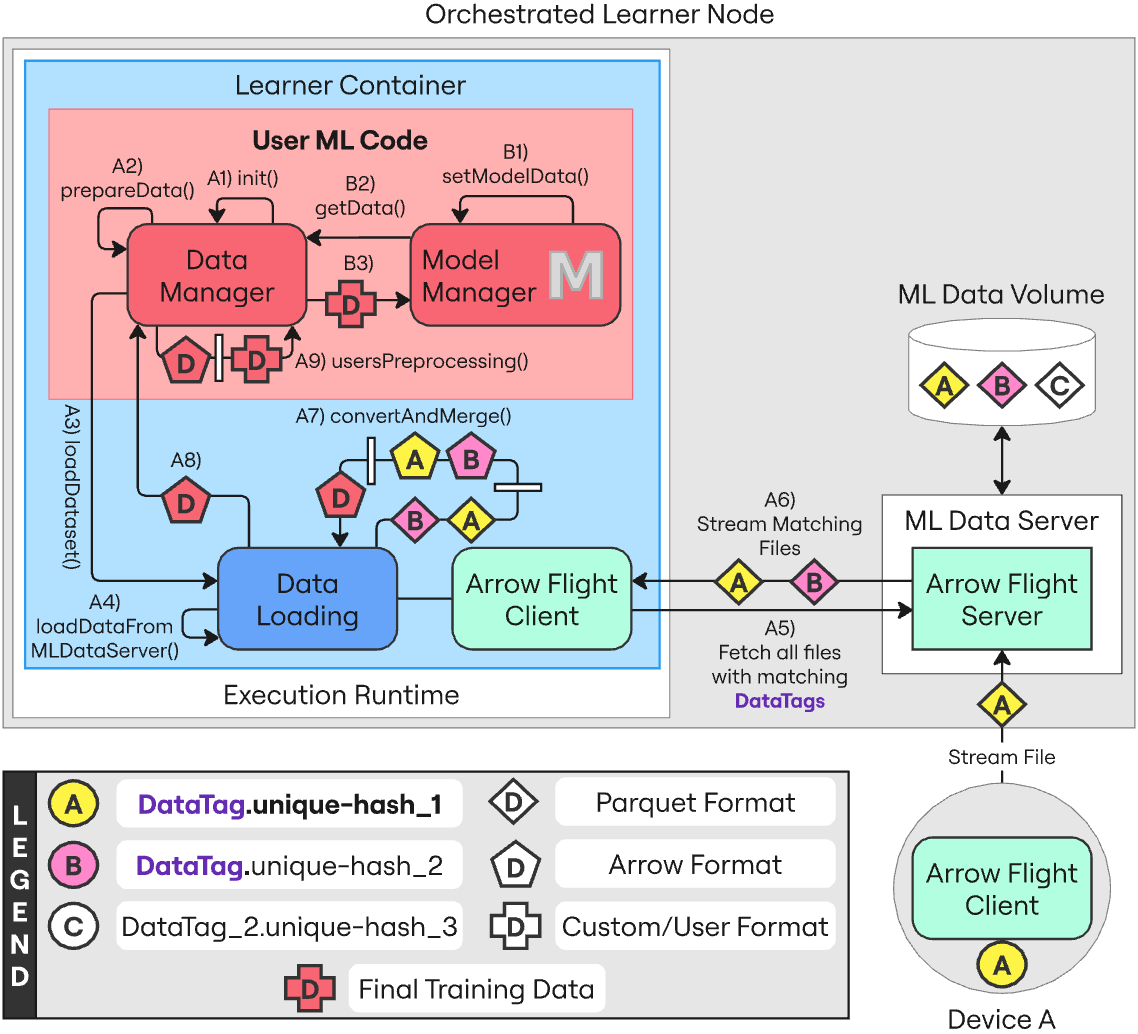
\includegraphics[width=0.90\paperwidth]{local_data_loading_detailed.png}
        \caption{Detailed FLOps Local Data Management Structure}
        \label{fig:detailed_local_data_management}
    \end{adjustwidth}
\end{figure}
Figure \ref{fig:detailed_local_data_management} depicts FLOps' local data management processes in more detail.
Firstly, the unique data resides on device A.
The device can store its data in an arbitrary format.
The device trusts the learner node in its proximity and transfers its data A to its ML data server via Flight.
For this, it needs to convert its data into Parquet format.
Secondly, the ML data server receives this streamed data and stores it locally on the learner node in a dedicated ML data volume.
This volume now contains several different Parquet files from different sources.
It uses Parquet files based on the last subsection's recommendations.

The next sequence of steps starts from the user's data manager.
During its initialization (A1), when the learner service is run, it triggers its \texttt{prepareData} function (A2).
This method calls the wrapper/adapter function \texttt{loadDataset} (A3).
The \texttt{loadDataset} function calls the \texttt{loadDataFromMLDataServer} function (A4).
This function is not available for users during development.
It is instead injected by the builder service, so it is exclusively available in the learner image's augmented FL code.

The Data Loading's \texttt{loadDataFromMLDataServer} function contacts its Flight client to request all matching files from the local ML data server (A5).
The match is performed based on the user's project SLA.
This SLA includes a \texttt{dataTags} key that is a list of string tags.
When devices send over their files, they must provide a data tag.
The ML data server will store these data files in the format seen in the Figure's legend.
The name starts with a singular data tag and ends with a unique hash based on the file's content.
Users and data providers need to cooperate to ensure that these data tags match.
The ML data server takes all files which name's prefix matches the user requested SLA data tags and streams them over into the learner container (A6).
In the example shown, only data files A and B have matching data tags.
The Flight server streams both over to the data-loading component.

Now that the matching data files are available inside the learner container, they must be transformed to fit the user's needs.
The data loading component converts its received Parquet files into Arrow format (A7) for better in-memory data management.
Usually, ML code expects and works with whole datasets instead of multiple split ones.
For this reason, the data loading component also merges its received files into a single dataset (A7).
The data loading component then sends this dataset to the user's data manager (A8).
The data manager now has access to the necessary dataset and can perform custom preprocessing and transformation steps (A9).
Users can freely configure and implement this preprocessing to ensure the retrieved data is usable for their ML model.

When FL training starts, the user's model manager will initially set the model data (B1).
Its \texttt{getData} method (B2) contacts the data manager and returns its prepared compatible dataset (B3).
In conclusion, these steps enable FLOps to manage and provide real local FL data to diverse user ML code for training and evaluation.

\subsection{Mock Data Providers}

Coordinating and managing real data providers while developing or testing can be challenging.
FLOps offers its own mock data providers to make these processes more convenient.
These optional services can be deployed on learner nodes via the orchestrator.
They split datasets into partitions and send them to the ML data server exactly as real devices.
It is enough to run them once to populate the local learner nodes with data.
These mock data providers also act as implementation examples for real devices when converting data, setting up a Flight client, and communicating with an ML data server.
The code is available here \cite{flops_code}.
Subsection \ref{subsection:api} shows the API endpoint for creating such mock data providers.
The FLOps Helper SLA for mock data providers looks as follows:
\begin{lstlisting}
    {   % The ID has to match the user's orchestrator ID.
        "customerID": "Admin",
        "mock_data_configuration": {
            % This value can be any dataset name available in Hugging Face.
            "dataset_name": "cifar10",
            "number_of_partitions": 1,
            "data_tag": "cifar10" 
        }
    }
\end{lstlisting}
\begin{figure}[h]
    \begin{adjustwidth}{-0.1\paperwidth}{-0.1\paperwidth}
        \centering
        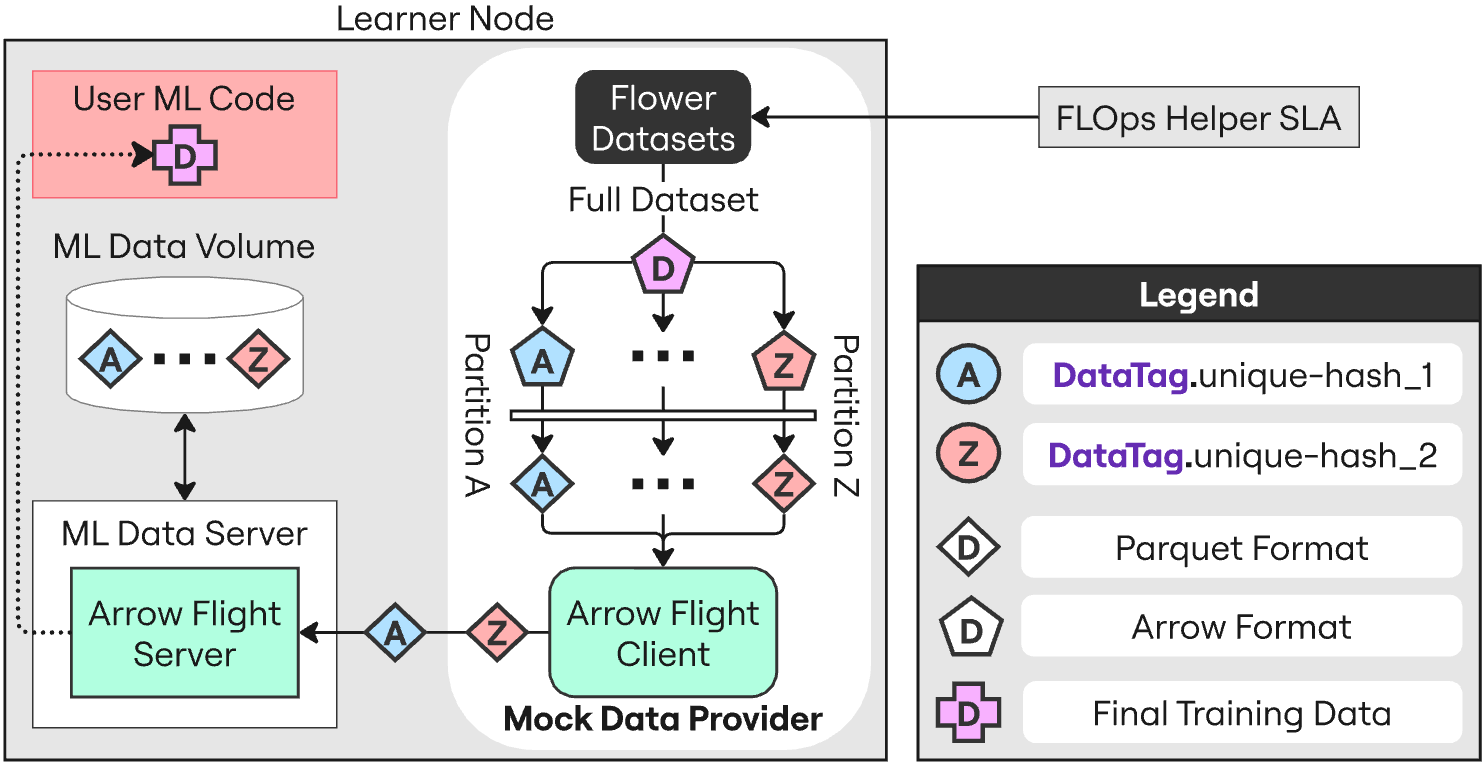
\includegraphics[width=0.80\paperwidth]{mock_data_provider.png}
        \caption{FLOps' Mock Data Provider}
        \label{fig:mock_data_provider}
    \end{adjustwidth}
\end{figure}
Figure \ref{fig:mock_data_provider} depicts FLOp's mock data provider.
The mock data provider runs as an orchestrated service in the container execution environment, similar to the learner service.
It uses the requested Hugging Face dataset name to download the dataset via Flower Datasets.
The data provider uses Flower Datasets to split this monolith dataset into multiple partitions.
The user defines the number of partitions.
Each partition is individually sent to the ML data server as if real edge devices were contacting the server.
The ML data server stores each partition separately in the ML data volume.
Ultimately, these partitions will be merged and preprocessed to be fit for training.



\section{MLOps via MLflow}

This section showcases how FLOps enables MLOps.
The first subsection discusses its MLOps components and how they work together.
The second subsection shows briefly how the GUI looks and works.
Many details were already mentioned in previous parts of this work.
Thus, this subsection will not repeat them but provide new insights or concretions.

\subsection{MLOps Components \& Architecture}

\begin{figure}[h]
    \centering
    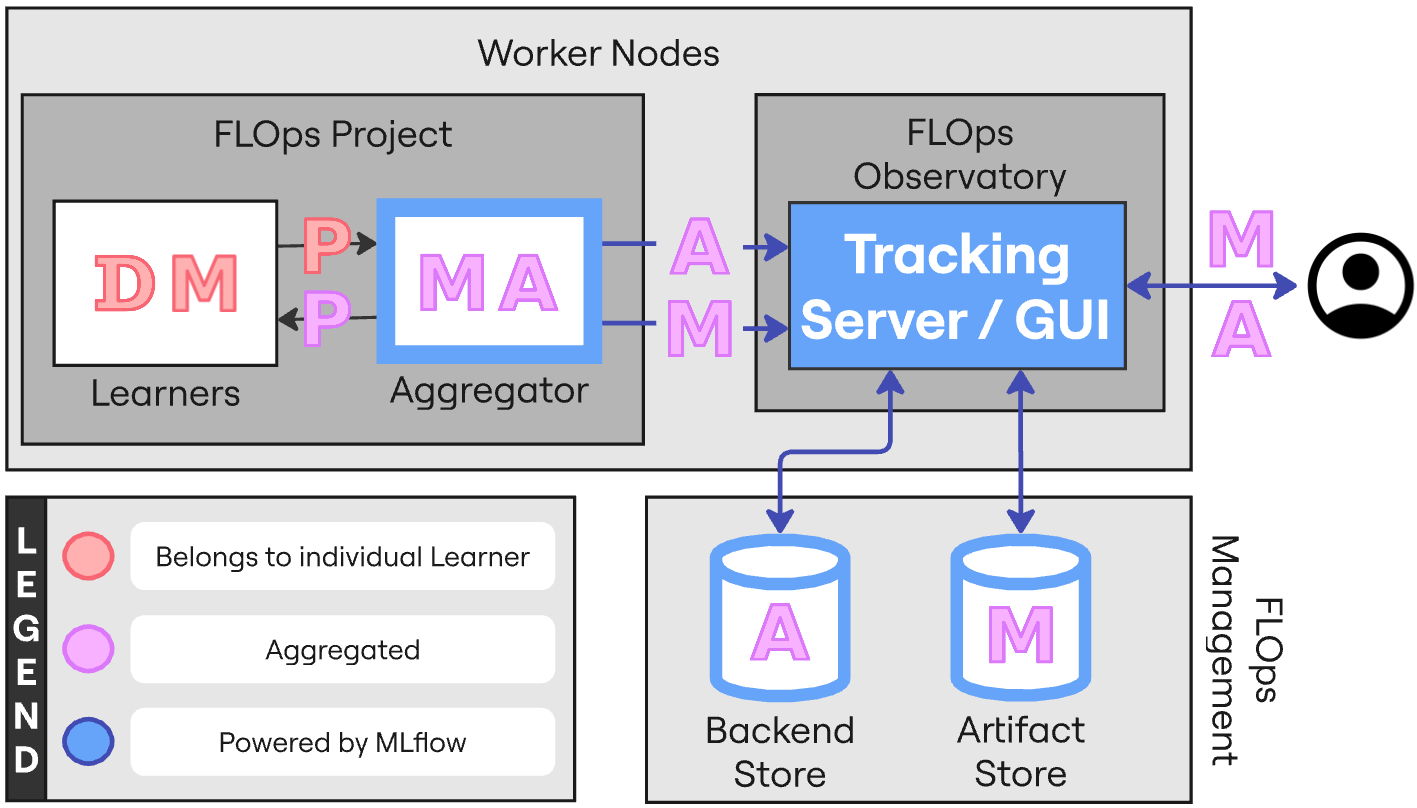
\includegraphics[width=1.0\textwidth]{mlops_components.png}
    \caption{FLOps' MLOps Architecture}
    \label{fig:mlops_architecture}
\end{figure}

This subsection builds on top of the discussed MLflow background (\ref{subsection:mlflow}) and subsystem decomposition (\ref{subsection:subsystem_decomposition}).

Figure \ref{fig:mlops_architecture} shows FLOps' MLOps architecture.
MLflow powers many FLOps' MLOps capabilities.
After every training round, the aggregator logs lightweight artifacts like metrics, parameters, tags, or runs.
In addition, the aggregator stores exactly one global model copy locally.
After every round, the aggregator checks if the new model's performance is better or worse.
The aggregator will update its local model if the new model is better.
At the end of the last training round, the aggregator sends the best trained global model to the artifact store.

An MLflow run represents an individual execution of (usually ML) code.
Each run can collect various pieces of information, such as metrics, hyperparameters, or custom tags.
These lightweight elements are represented as A in the Figure.
An MLflow experiment gathers multiple runs.
FLOps maps these MLflow terms directly to FL.
An experiment becomes an FLOps project and runs are FL training rounds.

The aggregator logs everything besides local elements over the tracking server. 
The tracking server works as a proxy for artifacts.
Thus, any access to any logged objects goes through the tracking server.
The tracking server itself does not have any state.
Its GUI showcases the stored elements in the backend and artifact stores hosted via the FLOps management.
Note that these stores can be deployed and scaled individually onto different machines.
There are various ways of setting up and provisioning MLflow components.
For example, the backend store can be a local directory, a remote database, a cloud file server, or blob storage.
The backend store hosts lightweight elements, and the artifact store hosts heavy-weight elements such as models or images.
FLOps currently uses a MySQL database for the backend store and a vsftpd (very secure FTP daemon) server for the artifact store.

It is noteworthy that no MLOps logging takes place on the learners.
Only the aggregator uses these techniques.
This approach works as expected regarding concrete FL metrics and models.
MLflow also provides a way to track system metrics, which FLOps uses.
These metrics only capture information about the aggregator, not the connected learners.
No information belonging to individual learners gets logged.
Furthermore, FLOps ensures that users can only access their own recorded artifacts.
FLOps explicitly upholds these separations to minimize possible privacy hazards and attack vectors.

\subsection{GUI}

FLOps uses MLFlow's GUI and does not modify it.
Therefore, this chapter only provides a brief selection of impressions of the GUI.
Excellent further details are available directly at MLflow \cite{mlflow:homepage}.

\begin{figure}[p]
    \begin{adjustwidth}{-0.1\paperwidth}{-0.1\paperwidth}
        \centering
        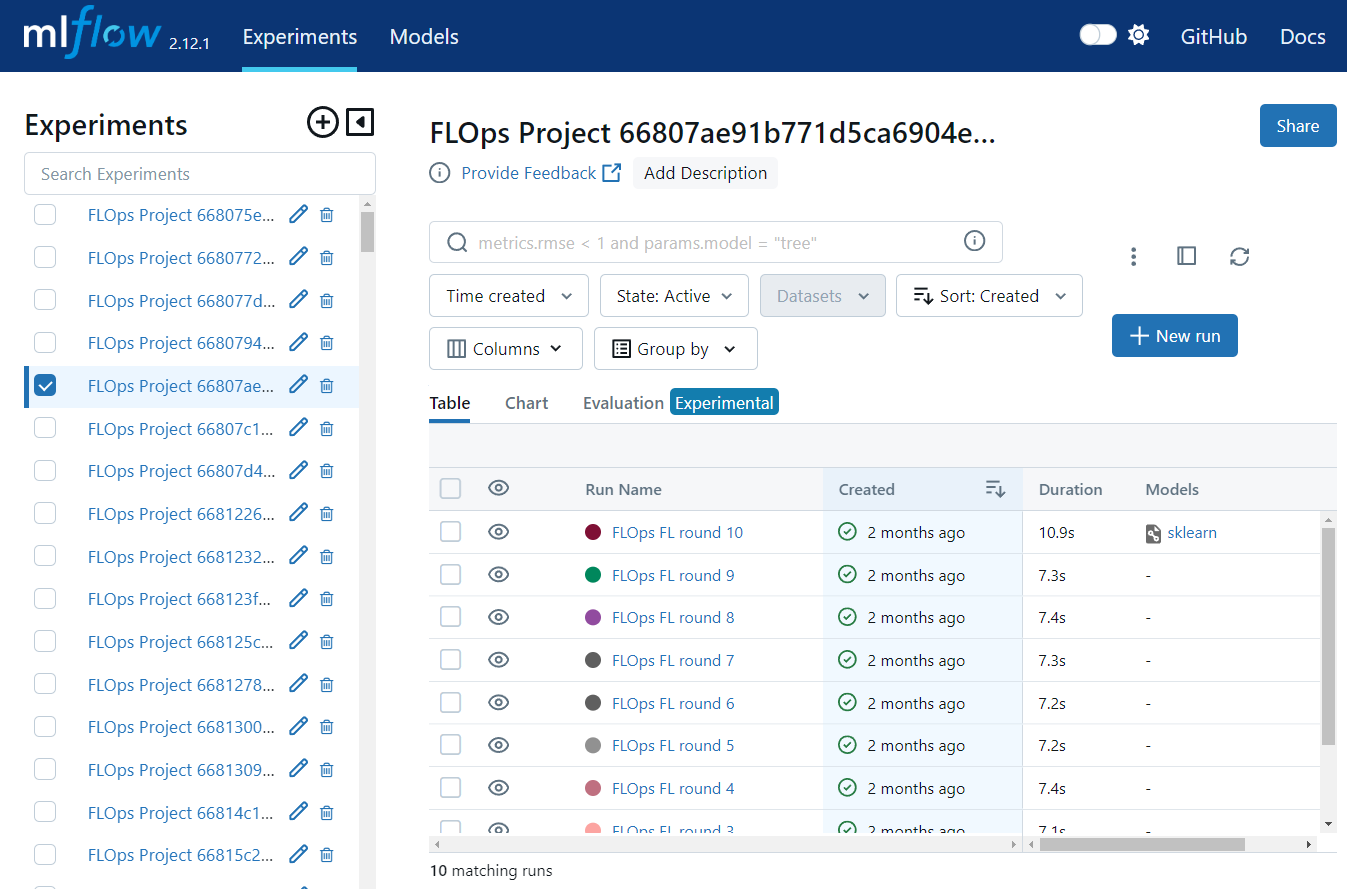
\includegraphics[width=0.90\paperwidth]{gui_ss_1.png}
        \caption{MLflow's GUI Screenshot - Experiments Overview}
        \label{fig:gui_ss_1}
    \end{adjustwidth}
\end{figure}

The first screenshot \ref{fig:gui_ss_1} shows MLflow's experiments overview page.
The left column lists all recorded experiments/projects.
Only a single one is currently selected.
Details about it are displayed to the right.
Multiple experiments can be selected simultaneously to view their combined contents.
The centerpiece offers a table view of the different FL rounds.
Users can customize and sort this table to their liking.
Each table row depicts a single FL round, when it was recorded, and its duration.
Only the best round contains a logged model.
In this example, the best round was the last (10th) round.

\begin{figure}[p]
    \begin{adjustwidth}{-0.1\paperwidth}{-0.1\paperwidth}
        \centering
        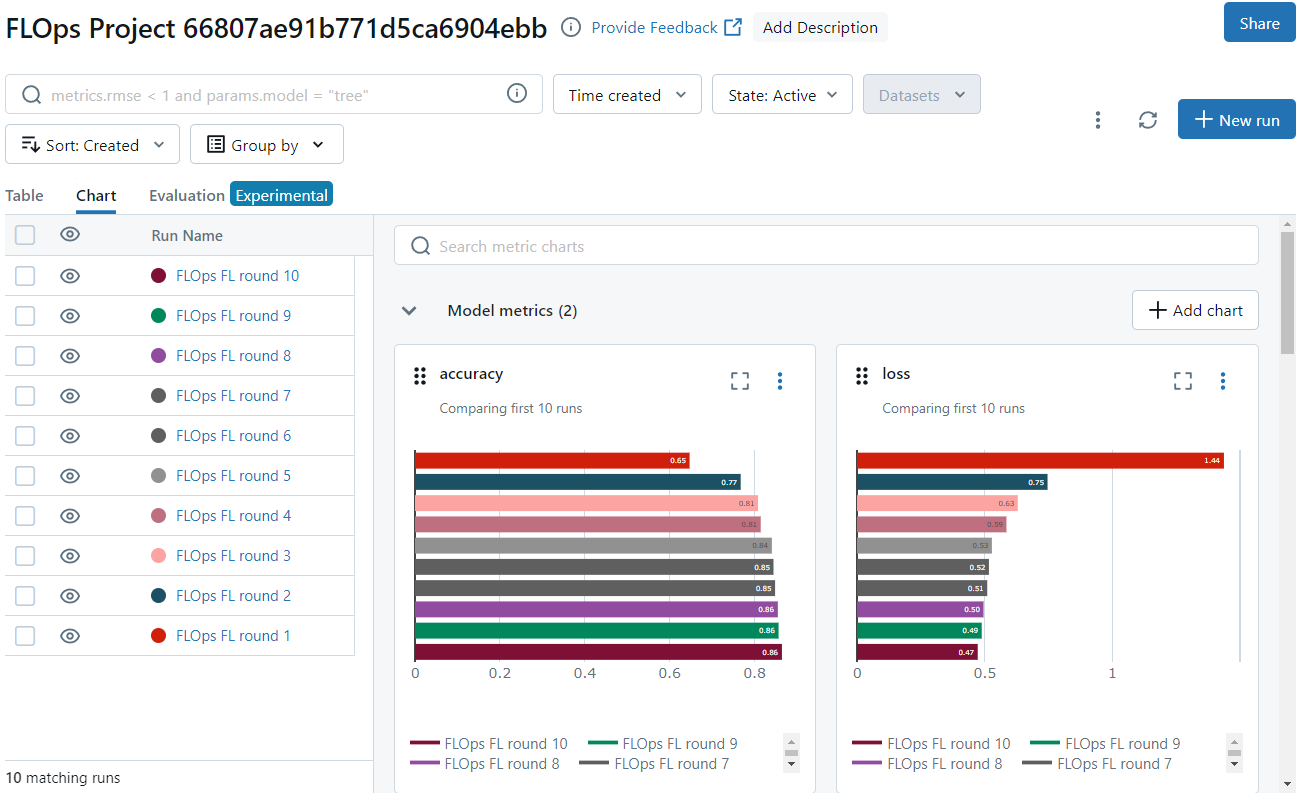
\includegraphics[width=0.90\paperwidth]{gui_ss_2.png}
        \caption{MLflow's GUI Screenshot - Experiment Details}
        \label{fig:gui_ss_2}
    \end{adjustwidth}
\end{figure}

Figure \ref{fig:gui_ss_2} shows the detailed view of a single recorded experiment/project.
Currently, FLOps focuses on the model's accuracy and loss.
The centerpiece of the screenshot shows the evolution of both across different FL rounds.
It shows that the model's accuracy improved, and its loss decreased over time.
FLOps users can access this GUI during FL training and observe how this FL-rounds table grows in real-time.

\begin{figure}[p]
    \centering
    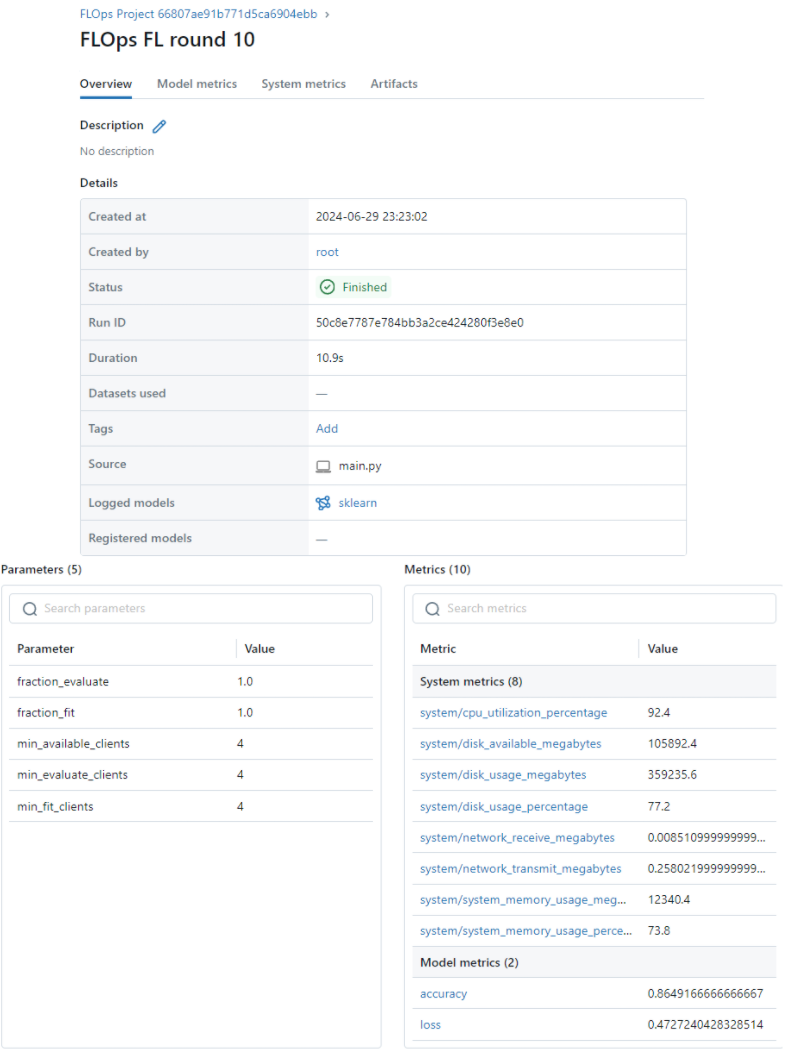
\includegraphics[height=1.0\textheight]{gui_ss_3.png}
    \caption{MLflow's GUI Screenshot - FL Round Details}
    \label{fig:gui_ss_3}
\end{figure}

The third screenshot \ref{fig:gui_ss_3} depicts concrete FL round details.
These details include general information such as if and what model was recorded, the run/round ID, or when the run was created.
In addition, it displays custom parameters that FLOps injected, including the user-provided number of clients/learners via the SLA.
This page also displays other metrics, such as accuracy or system metrics.

\begin{figure}[p]
    \begin{adjustwidth}{-0.1\paperwidth}{-0.1\paperwidth}
        \centering
        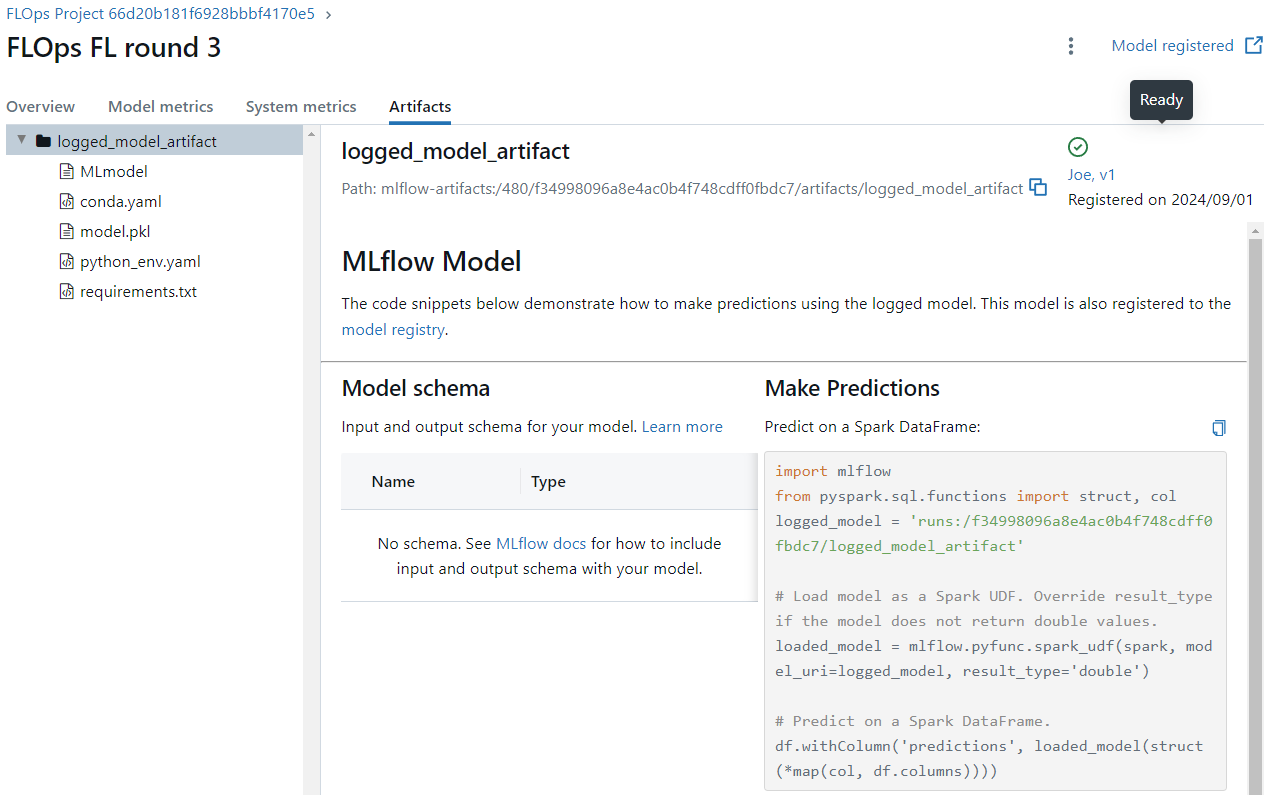
\includegraphics[width=0.90\paperwidth]{gui_ss_4.png}
        \caption{MLflow's GUI Screenshot - Logged Model Details}
        \label{fig:gui_ss_4}
    \end{adjustwidth}
\end{figure}

The last screenshot \ref{fig:gui_ss_4} shows the logged model details page.
The left folder shows the different aspects that were recorded.
The model requirements, conda environment, and model (pkl) file are all present.
This concrete example showcases a registered model (\ref{subsection:mlflow}).

MLflow is a feature-rich and well-documented MLOps tool.
Its GUI directly supports in-build techniques to compare, analyze, and visualize these logged results.
All of these recorded properties can be exported and shared with other people.
This thesis does not cover or use all MLflow's (GUI's) features.
Further information is available here \cite{mlflow:homepage,mlflow:docs}.

\section{Clustered HFL}

Besides classic FL, FLOps supports (clustered) HFL.
Oakestra's three-tiered layout supports geographically dispersed clusters.
Each cluster has its own cluster orchestrator and set of worker nodes.
This structure naturally alludes to the use of clustered and hierarchical FL.
Remembering Figure \ref{fig:uml_project_aggregators_analysis_object_model}, FLOps uses two different types of aggregators for HFL.
The root and cluster aggregators are deployed as services on worker nodes to distribute computational load.
Only a single root aggregator exists.
It can reside in any cluster.
Each orchestrated cluster hosts a single cluster aggregator.
A cluster aggregator only works with learners inside the same cluster.
This type of geographic clustering is why FLOps' HFL is a clustered approach.
Root aggregators treat cluster aggregators as plain learners, precisely as in classic FL.
Cluster aggregators are a combination between learner and aggregator.
Note that Flower does not natively support HFL.
Therefore, this approach of realizing HFL via Flower is a custom novel solution.

\begin{figure}[p]
    \begin{adjustwidth}{-0.1\paperwidth}{-0.1\paperwidth}
        \centering
        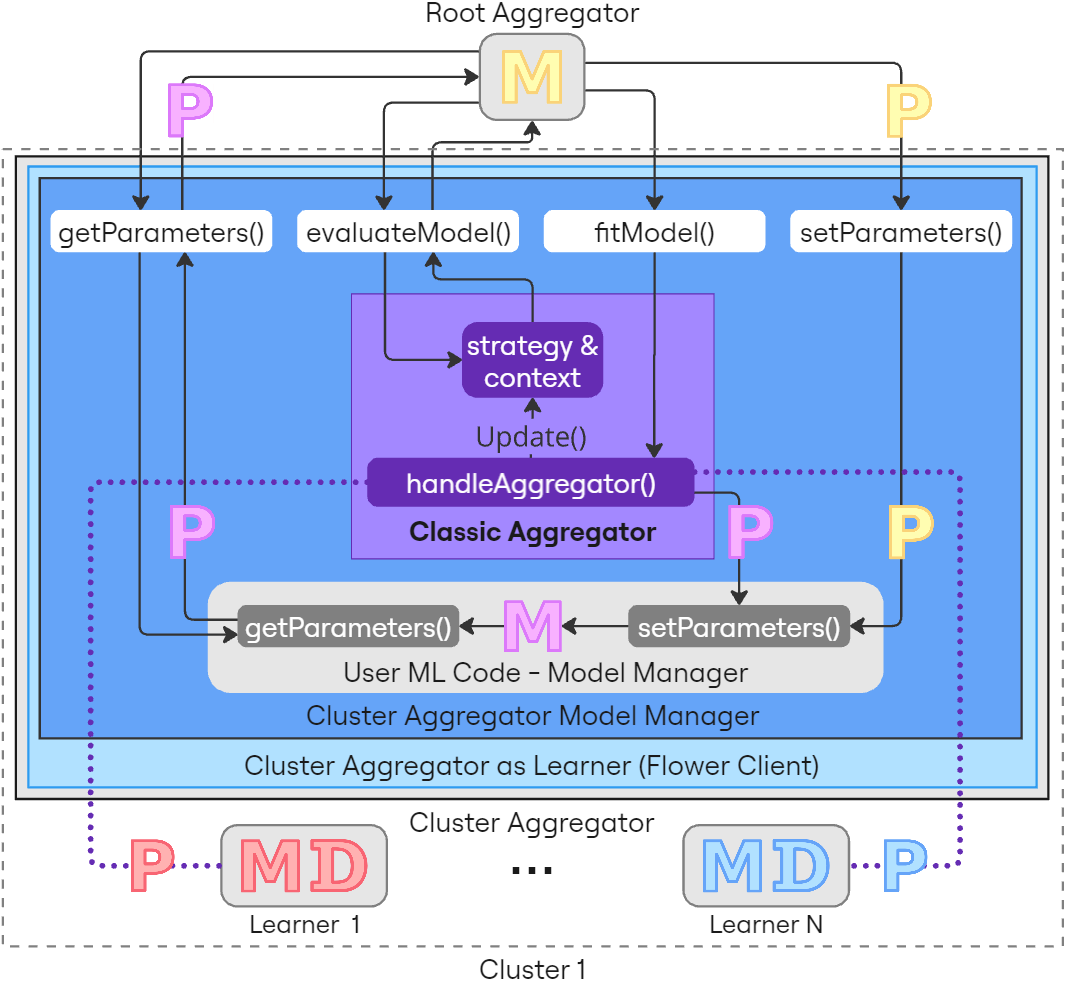
\includegraphics[width=0.80\paperwidth]{clustered_hfl_architecture.png}
        \caption{FLOps clustered HFL Architecture}
        \label{fig:flops_clustered_hfl_architecture}
    \end{adjustwidth}
\end{figure}
Figure \ref{fig:flops_clustered_hfl_architecture} shows the detailed architecture of how FLOps realizes clustered HFL.
This figure reuses and expands upon the stylistic conventions seen throughout this thesis, starting from Figure \ref{fig:basic_fl_intro}.
Every visible element beside the root aggregator is part of a single cluster.
This setup supports multiple clusters.
Because the root aggregator interacts with the cluster aggregators as if they were plain learners, cluster aggregators need to offer the same learner interface.
The cluster aggregator implements the same learner interface and model manager as user ML code repositories.
This approach requires implementing this interface properly and maintaining the state during multiple training cycles.
Therefore, the cluster aggregator needs to be able to modify and access the underlying user ML model.
This model is the main reference point for model parameters in a cluster aggregator.

At the start of a new training cycle the root aggregator calls the cluster aggregator's \texttt{fitModel} method.
It triggers the cluster aggregator's \texttt{handleAggregator} method, which all aggregator types in FLOps have.
The cluster aggregator performs conventional FL training with its learners and fuses new intermediate global parameters (pink P).
Then, it updates its model copy stored in the user's model manager.
By default, Flower also evaluates the model during training.
The custom FLOps aggregator strategy can store and accumulate evaluation results.
When the root aggregator requests to evaluate the cluster aggregator, it retrieves the stored values from the strategy and context objects.
When the root aggregator calls the cluster aggregator's \texttt{getParameters} method, the cluster aggregator calls its user's model manager \texttt{getParameters} method.
The same applies to setting parameters.

In other words, the cluster aggregator mimics a learner by using the same interface, which works on the same user-provided ML model.
The main differences between a learner and the cluster aggregator are that the fit model method performs classic FL training rounds, the evaluate function retrieves recorded results from the aggregator objects, and that the aggregator has no access to data.
This way, FLOps can perform clustered hierarchical FL.
Note that the underlying code is shared among all aggregator types, thus avoiding several similar implementations.
I.e., the same aggregator image gets deployed with different parameters that decide the aggregator's behavior.


\section{CLI}

While developing FLOps, we implemented several different pieces of code to automate tedious, repetitive manual tasks.
We decided to share and offer these custom auxiliary scripts by combining them into a single CLI tool called OAK CLI \cite{cli_code}.
We have steadily improved it over this work, which resulted in various features.
Because of the envisioned rapid changes in the future, we will not discuss concrete technical details but provide a broad overview of its capabilities.
We decided to discuss this CLI as part of this work because FLOps can be considered DevOps for FL, and DevOps also includes techniques to improve development workflows.
One way to support users and developers is to help them use the target application more conveniently, for example, via a CLI tool.
Notably, Oakestra has a custom early-stage work-in-progress GUI/Frontend dashboard application \cite{oakestra_dashboard} and a minimal CLI tool.
The OAK CLI is independent of both these components and replaced the legacy Oakestra CLI tool.

We were motivated to create this CLI to alleviate the following challenges.
FLOps does not offer a tool besides the OAK CLI to interact conveniently with its API.
External tools like Postman are necessary to do so.
Oakestra components need to be prepared and launched manually.
Interacting with its API is possible via external tools or its early-stage dashboard.
We needed to work on several devices while developing FLOps, especially its HFL features.
Each machine must be appropriately configured and set up to enable Oakestra workloads.
This setup included installing dependencies such as Docker, Golang, and other custom aliases and scripts to launch, clear, and restart Oakestra components.
In addition, developing and observing FLOps was heavily bound to the observatory features provided by Oakestra's dashboard application.
Accessing and working with this dashboard was cumbersome even during local development on a single machine because of repetitive click-based tasks such as mandatory logins.
We automated this by creating auto-clicker scripts via Selenium.
Accessing this flaky dashboard on remote devices behind firewalls required even more manual steps, such as code modifications and multiple SSH tunnels.
We only required the dashboard to get an overview of the deployed application and services and their statuses and logs.
The OAK CLI satisfies these needs independently, bypassing our need for the dashboard while automating manual steps.
As a result, this CLI significantly accelerates the development and usage of FLOps and Oakestra.

\subsection{CLI Requirements Discussion}

The OAK CLI needs to satisfy the following requirements:
\vspace{5mm}
\newline
\textbf{Interface for APIs}\newline
The CLI should interact with the APIs of FLOps and Oakestra to alleviate the need for users to use external tools, know all API endpoints, and know how to interact with them appropriately.
The key activities the CLI should support are managing applications and services in Oakestra and starting projects in FLOps.
For example, if the user wants to create a new application in Oakestra he first needs to login.
For the login, the user needs to know the login URI, create a fitting request, send it, and extract the received bearer token for authentication and authorization.
Only afterward can users prepare their application SLA, add their token, and send it to the application POST endpoint.
Instead, the CLI should offer a single command so that users only need to provide their application SLA. 
The CLI will perform the login and handle the API interactions.
\vspace{5mm}
\newline
\textbf{Observability}\newline
FLOps handles many different applications and services concurrently.
Especially during development, it is crucial to observe whether components behave as expected and identify unexpected errors or behavior as quickly as possible.
For this, the CLI needs to provide its users with an overview of the current state of applications and deployed services.
This overview should include comprehensive information about these components, such as their current status, critical properties, and details.
It is crucial to provide timely information to the user.
The CLI should support a way to observe the current situation close to real-time.
\vspace{5mm}
\newline
\textbf{Accelerated Workflows via Automation}\newline
The more manual, tedious, repetitive tasks can be accelerated via automation, the more high-quality work can be done and less frustration generated.
The tool should provide ways of installing dependencies to make Oakestra's and FLOps' setup quicker and easier on new machines.
The CLI should handle starting, stopping, restarting, and rebuilding Oakestra and FLOps components to speed up and simplify development cycles.
In addition, it should be a common place to host valuable additions from different individuals, including aliases or scripts.
The CLI should be easily modified and extended to accompany future user demands.
\vspace{5mm}
\newline
Based on these requirements, it is easy to see that this singular tool has many responsibilities to uphold and features to offer.
These features are of no equal interest to all its possible users.
Casual end-users require and demand other features than administrators or developers.
The usable feature set is also heavily dependent on the machine on which the CLI runs.
A machine can be a standalone control plane that only includes the root or cluster orchestrators.
It can be a standalone worker node or a hybrid of several scenarios.
A machine can also simultaneously include all these mentioned components and be a monolith system.
All these options require different needs and, conversely, do not require all features or are not capable of or intended to provide all features.
For example, a worker node should be unable to restart the root orchestrator, whereas the root orchestrator should not be able to tinker with sensitive worker node configurations.

A tool that fulfills all mentioned requirements can be divided into several, one for each use case or provided by a dynamic large single tool.
Multiple tools have the benefit of being less overwhelming, leading to smaller and tidier repositories, and users do not need to understand the big picture.
The downside of multiple tools is the risk of entangled and divergent dependencies that need to be managed.
Such tools will still show interdependencies and coupling, leading to split comprehension.
Users, especially developers, would need to know exactly what tool is responsible for what and how they are interconnected, potentially making things more complex.
With split tools, there is the risk of increased code duplication over time, especially if different people develop different parts without understanding related tools.
The benefit of a single tool is that everything is in one place and forms a single source of truth.
Developers can efficiently work with a single well-structured repository.
Users only need to install and update a single tool instead of several.
Code and logic can be more easily reused between the same code base.
The downsides of a single tool are the risk of high coupling and increased complexities as the project grows.
OAK CLI is a single tool because we explicitly structured it to support low coupling and high cohesion.
Its flexible design enables easy separation and extension.
Thus, all FLOps-specific functionalities can be easily isolated and converted into a separate CLI tool.
We aim towards a modular monolith design that suits a smaller team like ours.

\subsection{High Level CLI Details}

The CLI can create, delete, and (un)deploy applications and services.
It can present current information about available apps and services in different verbosity levels.
In addition, it allows to inspect latest service logs.
Users can use the CLI to manage FLOps components, including its manager, database, projects, and tracking server.
The CLI automates tedious manual tasks such as clearing local images or rebuilding orchestrator components.
It can install fundamental dependencies such as Docker and Golang.
The CLI has a customizable config file that allows users to specify their intended use case and filter out unwanted commands.
It also features experimental commands to run automatic evaluations.
Detailed descriptions of the CLI commands and options with screenshots are available in the appendix \ref{appendix:cli}.

